\scanpage{83}
% archive sheet number: 82
% Long oblique strokes cancel this draft.
\deleted{IV 7.5.}

\deleted{Je ne suis pas très content encore de la dernière version, car on n'énonce pas ce qu'on démontre vraiment, et par conséquent il y a des cas (tels la ``$\text{\unsure{\rlap{p}c}\unsure{\rlap{r}o}p\rlap{f}rof}\quad n$'', ou ``in\rlap{è}tègre'') qui échappent à l'énoncé tel qu'il est donné, mais sont inclus dans la démonstration. Aussi je propose de réénoncer les choses ainsi:}

\deleted{\uline{Théorème} 7.5.1.\quad Soit $A\quad B$ un homomorphisme local d'anneaux locaux noéthériens, $\text{\uuline{R}}(C)$ une propriété \deleted{d'anneaux locaux} faisant intervenir un argument qui e st un anneau local noe\rlap{h}t\unsure{\rlap{t}h|h}érien. On suppose\deleted{\unsure{x|r}} que $(B,R)$ satisfait à :}

\deleted{a) Pour tout anneau \mbox{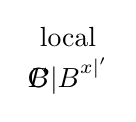
\begin{tikzpicture}[baseline=(base.base)]
\node[inner sep=0] (base) {$\text{\unsure{\rlap{C}B|B}}^{\deleted{\unsure{x|'}}}$};
\node[anchor=south,inner sep=0,yshift=.12cm] at (base.north) {\inserted{local}};
\end{tikzpicture}} localise d'une $B$-algèbre finie, et tout élément régulier $t\quad\underline{r}(C)$, $\text{\uuline{R}}(C/tC)$ implique $\text{\uuline{R}}(C)$.}

\deleted{b) Si $C$ est une $B$-algèbre finie, alors $U_{\text{\uuline{R}}}(\operatorname{Spec}(C))$ est ouvert.}

\deleted{On suppose de plus que $A$ satisfait les conditions suivantes\deleted{\unsure{x}} (remplies si $A$ est ``excellent'' (7.8.2.) en particulier si $A$ est complet):}

\deleted{\handwritten{$\alpha$}) $A$ est \mbox{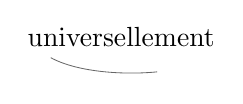
\begin{tikzpicture}[baseline=(word.base)]
\node[inner sep=0] (word) {universellement};
% Thin shallow curved trace below the first half; no textual value or origin assigned.
\draw[line width=.3pt,opacity=.6] ([xshift=.30cm,yshift=-.13cm]word.south west) .. controls ([xshift=.65cm,yshift=-.32cm]word.south west) and ([xshift=1.25cm,yshift=-.35cm]word.south west) .. ([xshift=1.65cm,yshift=-.31cm]word.south west);
\end{tikzpicture}} japonais.}

\deleted{\handwritten{$\beta$}) Pour toute algèbre finie intègre $C$ sur $A$, $\operatorname{Spec}(C)$ contient un ouvert non vide qui est régulier,}

\deleted{\mbox{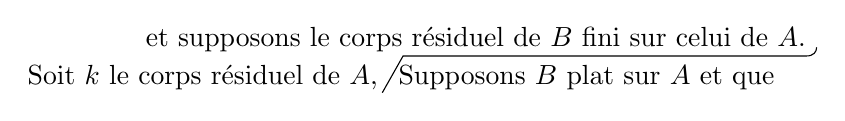
\begin{tikzpicture}[baseline=(left.base)]
\node[inner sep=0] (left) {Soit $k$ le corps résiduel de $A$,};
\node[anchor=base west,inner sep=0,xshift=.25cm] (right) at (left.base east) {Supposons $B$ plat sur $A$ et que};
\node[anchor=south west,inner sep=0,xshift=1.5cm,yshift=.15cm] (added) at (left.north west) {\inserted{et supposons le corps résiduel de $B$ fini sur celui de $A$.}};
\path (added.south west) -- coordinate[pos=.39] (bend) (added.south east);
\draw ([xshift=.05cm,yshift=-.03cm]left.south east) -- ([yshift=-.04cm]bend) -- ([yshift=-.04cm]added.south east) .. controls ([xshift=.09cm,yshift=-.04cm]added.south east) and ([xshift=.13cm,yshift=.01cm]added.south east) .. ([xshift=.13cm,yshift=.07cm]added.south east);
\end{tikzpicture}} $B\otimes_A k$ sur $k$ satisfait la condition ``$Q$ géométrique''; \rlap{a}Alors toutes les fibres de $\operatorname{Spec}(B)$ sur $\operatorname{Spec}(A)$ satisfont la condition $Q$ géométrique.}

\deleted{Démonstration. Les hypothèses faites sur $A\quad B$ sont stables par changement de base fini $A\quad A'$, pourvu qu'on prenne soin de ref\unsure{\rlap{r}o}rmuler les hypothèses pour $A,B$ semi-locaux, l'homomorphisme $A\quad B$ semi-local (i.e. l'image inverse d'un idéal maximal est un idéal maximal) et qu'on remplace le corps résiduel de $A$ par les corps résiduels de $A$. \deleted{(NB alors} (NB cette extension ne mérite pas de figurer dans l'énoncé du théorème, c'est juste un intermédiaire technique pour la démonstration). On est ainsi ramené au cas $A$ intègre et à voir que la fibre générique satisfait}
